\chapter{Requirements Specification}
\label{ch:requirements}

\section{System Context, Stakeholders, Assumptions, and Constraints}
\label{sec:context}

InfraArchAgent is a standalone web application that generates security-scanned
candidate AWS infrastructure from natural-language descriptions. It sits between
the engineer's intent and the IaC files that intent requires, automating the
authorship and security validation steps that currently demand hours of
multi-tool expertise.

\subsection*{System Boundary}

The system boundary encloses a React frontend, a Python backend hosting the
agent pipeline, and a PostgreSQL database. Everything outside the boundary,
the LLM API, Checkov and tfsec binaries, and the engineer's AWS environment,
is an external dependency. The system generates files; it does not execute
them. No cloud credentials enter the system at any point.

\subsection*{Actors}

\begin{description}[leftmargin=3cm, style=nextline]
  \item[DevOps Engineer] The primary user. Submits natural-language
    infrastructure descriptions, monitors pipeline execution, reviews
    generated packages, and downloads the chosen variant.
  \item[LLM API] External AI service (Claude or GPT-4o) that the four
    agents call to perform reasoning and generation tasks.
\end{description}

\subsection*{External Systems}

\begin{itemize}
  \item \textbf{LLM API} (Anthropic Messages API or OpenAI chat completions):
    receives structured JSON prompts from agents and returns structured JSON
    responses.
  \item \textbf{Checkov}: static analysis tool invoked as a subprocess to
    scan generated Terraform and Kubernetes files for security
    misconfigurations.
  \item \textbf{tfsec}: static analysis tool invoked as a subprocess to
    scan generated Terraform files for AWS-specific vulnerabilities.
\end{itemize}

\subsection*{Assumptions}

\begin{itemize}
  \item Each LLM call allows 30 seconds per attempt with exponential backoff
    across up to 3 attempts; the total per-agent LLM deadline is 150 seconds
    under normal operating conditions.
  \item The engineer's input is written in English and describes
    infrastructure that is technically feasible on AWS.
  \item Checkov 3.x and tfsec 1.x are installed and accessible in the
    backend runtime environment.
  \item The engineer reviewing the output has sufficient IaC knowledge to
    evaluate the generated files before deploying them.
\end{itemize}

\subsection*{Constraints}

\begin{itemize}
  \item Generated IaC targets AWS resource types only; Azure and GCP are
    out of scope.
  \item The system has no offline generation capability; LLM API access
    is required for all pipeline runs.
  \item The system holds no cloud credentials and cannot apply, plan, or
    destroy infrastructure against any provider.
  \item The backend runtime requires Python 3.11 or later; the frontend
    build requires Node.js 18 or later.
  \item \textbf{Single-user prototype.} InfraArchAgent is designed as a
    single-user local deployment. No multi-user authentication, session
    management, or run ownership model is implemented. Multi-user support
    is a non-goal for this thesis.
  \item \textbf{Human-in-the-loop production readiness.} InfraArchAgent
    automatically labels a package \texttt{production\_ready} only when
    the SecurityAgent resolves all violations without human intervention
    and the package then passes validation. Packages that exhaust the
    remediation iteration limit, fail validation, or are left without a
    validation report because the ValidatorAgent crashed enter
    \texttt{pending\_review} and require an explicit engineer decision
    (approve, retry with feedback, or reject) before being labelled
    \texttt{production\_ready} or \texttt{not\_production\_ready}. No
    package is ever silently delivered without a definitive readiness
    label.
\end{itemize}

\subsection*{Pipeline State and Timing Model}

\begin{longtable}{@{}p{0.20\textwidth}p{0.25\textwidth}p{0.25\textwidth}p{0.20\textwidth}@{}}
\caption{Pipeline run states and timing constraints.}\label{tab:states}\\
\toprule
\textbf{State} & \textbf{Meaning} & \textbf{Transition condition} &
  \textbf{Result cardinality} \\
\midrule
\endfirsthead
\toprule
\textbf{State} & \textbf{Meaning} & \textbf{Transition condition} &
  \textbf{Result cardinality} \\
\midrule
\endhead
\texttt{running} & Pipeline is executing & Input accepted & 0 packages \\
\texttt{success} & All agents completed cleanly & All 3 generators
  completed and every resulting package reached
  \texttt{production\_ready} automatically, with no violations requiring
  engineer review & 3 packages \\
\texttt{partial\_success} & At least one package available, but the run
  didn't finish cleanly & 1--2 generators completed; \emph{or} all 3
  completed but at least one package ended in \texttt{pending\_review}
  (because of unresolved security violations, a validation failure, or a
  validator crash) & 1--3 packages \\
\texttt{failed} & No usable output & ArchitectAgent failed after retries,
  all generators timed out, or every package hit \texttt{scan\_error} &
  0 packages \\
\bottomrule
\end{longtable}

Per-agent timing: each LLM call allows 30 seconds per attempt with
exponential backoff across up to 3 attempts (30s + 60s + 60s = maximum
150 seconds total per agent including backoff delays). The ArchitectAgent
end-to-end deadline is 150 seconds. Each GeneratorAgent end-to-end deadline
is 150 seconds. The full pipeline deadline is 5 minutes (PR-01), measured
to the point where the run reaches \texttt{success} or
\texttt{partial\_success}; time spent afterward in \texttt{pending\_review}
is not counted against this deadline, since it depends on the engineer, not
the pipeline. Partial success counts against PR-01 with available packages
only.

% ---------------------------------------------------------------------------
\section{Functional Requirements}
\label{sec:functional}

\begin{longtable}{@{}p{0.10\textwidth}p{0.42\textwidth}p{0.36\textwidth}@{}}
\caption{Functional requirements.}\label{tab:functional-requirements}\\
\toprule
\textbf{ID} & \textbf{Requirement} & \textbf{Acceptance evidence} \\
\midrule
\endfirsthead
\toprule
\textbf{ID} & \textbf{Requirement} & \textbf{Acceptance evidence} \\
\midrule
\endhead

FR-I-01 & The system shall accept a UTF-8 encoded natural-language string as
  the primary input for infrastructure generation (minimum 10 characters,
  maximum 2,000 characters). &
  Unit test: inputs at boundary lengths accepted; inputs outside rejected
  with HTTP 400. \\

FR-I-02 & The system shall reject inputs that contain no identifiable
  infrastructure intent and return HTTP 422 with a plain-English
  explanation. &
  Unit test: submit ``hello'' and similar non-infrastructure strings;
  verify 422 response and explanation text. \\

FR-I-03 & The system shall assign a unique run ID to every accepted pipeline
  request and persist it to the database before invoking the
  ArchitectAgent. &
  Integration test: confirm run ID exists in \texttt{pipeline\_runs}
  before ArchitectAgent call completes. \\

FR-I-04 & The system shall accept an optional configuration object specifying
  LLM provider, model identifier, and maximum remediation iterations;
  omitted fields default to system-configured values. &
  Integration test: run with and without configuration object; verify
  defaults apply when omitted. \\

\midrule

FR-A-01 & The ArchitectAgent shall parse the natural-language input and
  produce a structured deployment plan in JSON format covering target AWS
  services, component dependencies, network topology, and storage
  requirements. &
  Integration test: submit known input; assert plan JSON contains
  expected service names and dependency graph. \\

FR-A-02 & The deployment plan shall explicitly name every IaC file type
  required for the described infrastructure. &
  Unit test: parse plan output; verify file type list matches
  expected set for the given description. \\

FR-A-03 & The ArchitectAgent shall include an ambiguity note in the plan
  rather than silently assuming defaults when the input is underspecified. &
  Integration test: submit ``a web app'' with no runtime specified;
  assert plan contains an ambiguity field. \\

FR-A-04 & The ArchitectAgent end-to-end deadline is 150 seconds (30 seconds
  per LLM call attempt, up to 3 attempts with exponential backoff, maximum
  150 seconds total including backoff delays); exceeding this marks the run
  as failed. &
  Integration test with mocked LLM: simulate all retries exhausted;
  verify run status is \texttt{failed} and error is persisted. \\

FR-A-05 & The deployment plan shall be the sole input to all three
  GeneratorAgents; no GeneratorAgent shall read the original
  natural-language string directly. &
  Code review: assert GeneratorAgent constructors accept only plan dict,
  not raw input string. \\

\midrule

FR-G-01 & The system shall run exactly three GeneratorAgent instances in
  parallel, each receiving an identical copy of the deployment plan
  alongside a distinct optimisation directive (cost, performance,
  security). &
  Integration test: instrument async task launch; verify three concurrent
  tasks with distinct directives. \\

FR-G-02 & Each GeneratorAgent shall produce a complete IaC package
  containing all file types named in the deployment plan; incomplete
  packages shall not proceed to the SecurityAgent. &
  Integration test: mock one generator to omit a file; verify package
  is rejected before SecurityAgent call. \\

FR-G-03 & The cost-optimised GeneratorAgent shall prefer AWS Free Tier
  eligible resource types, smaller instance sizes, and on-demand pricing. &
  Integration test: inspect generated Terraform; verify instance type
  is \texttt{t3.micro} or equivalent Free Tier resource. \\

FR-G-04 & The performance-optimised GeneratorAgent shall prefer larger
  instance types, multi-AZ deployments, and autoscaling configurations. &
  Integration test: inspect generated Terraform; verify
  \texttt{multi\_az = true} and autoscaling group present. \\

FR-G-05 & The security-optimised GeneratorAgent shall apply the most
  restrictive IAM policies, enable encryption at rest and in transit,
  and prefer private subnets. &
  Integration test: run Checkov against security variant output; verify
  zero HIGH-severity violations on first scan. \\

FR-G-06 & All three GeneratorAgents shall complete within 150 seconds;
  individual failures are non-fatal provided at least one package
  completes. The run transitions to \texttt{partial\_success} if 1--2
  generators succeed. &
  Integration test: mock one generator to time out; verify pipeline
  continues with two packages and state is \texttt{partial\_success}. \\

FR-G-07 & Each generated package shall be stored to the database under the
  pipeline run ID before the SecurityAgent begins scanning. &
  Integration test: assert \texttt{generated\_packages} rows exist for
  run ID before SecurityAgent task starts. \\

\midrule

FR-S-01 & The SecurityAgent shall run Checkov and tfsec concurrently
  against every package produced by the GeneratorAgents. &
  Integration test: instrument subprocess calls; verify both tools
  invoked per package before any remediation begins. \\

FR-S-02 & The SecurityAgent shall attempt autonomous remediation for every
  violation reported and record each change as a diff against the
  pre-remediation version. &
  Integration test: inject a known violation; verify the violation is
  absent in the output and the diff records the change. \\

FR-S-03 & After remediating all violations in a pass, the SecurityAgent
  shall re-run both scanners; this loop continues until violations are
  resolved or the configured iteration limit is reached (default: 3). &
  Integration test: inject a violation that requires two remediation
  passes; verify the loop runs twice and exits clean. \\

FR-S-04 & The SecurityAgent shall persist the full scan report for each
  iteration to the database, including violation descriptions, file
  paths, line numbers, and the remediation applied. &
  Integration test: inspect \texttt{generated\_packages.security\_report}
  after a run; verify all required fields are present. \\

FR-S-05 & Packages that reach the iteration limit with unresolved violations
  shall proceed to the ValidatorAgent and be presented to the engineer
  with those violations clearly flagged. &
  Integration test: set max iterations to 1 with an un-fixable violation;
  verify package reaches the UI with violation flagged. \\

FR-S-06 & The SecurityAgent shall produce a unified diff for each package
  showing all changes made across all remediation iterations. &
  Integration test: inspect \texttt{generated\_packages.remediation\_diff};
  verify diff format is valid and covers all changed lines. \\

FR-S-07 & When the remediation loop exits with unresolved violations
  remaining, the SecurityAgent shall transition the package to a
  \texttt{pending\_review} state and halt further automated remediation
  until the engineer acts. A package shall also enter
  \texttt{pending\_review}, even if its scan was clean, when validation
  fails (\texttt{invalid}) or the ValidatorAgent cannot produce a report
  (\texttt{validation\_error}) (FR-V-05). A package is labelled
  \texttt{production\_ready} automatically only if its scan was clean and
  validation passed. &
  Integration test: force iteration limit exhaustion; verify package
  state is \texttt{pending\_review} and no further scan calls occur.
  Integration test: a clean-scan package whose validation fails ends in
  \texttt{pending\_review}; likewise for a clean-scan package whose
  ValidatorAgent crashes. \\

FR-S-08 & The engineer shall be able to approve a package in
  \texttt{pending\_review}, transitioning it directly to
  \texttt{production\_ready} without triggering a rescan. &
  UI test: click approve on a pending\_review package; verify state
  changes to production\_ready and no SecurityAgent call is made. \\

FR-S-09 & The engineer shall be able to request a remediation retry on a
  package in \texttt{pending\_review}, optionally supplying free-text
  feedback; the SecurityAgent shall reset the iteration counter to the
  full configured limit (i.e.\ the count of iterations already consumed
  returns to zero) and include the feedback, together with any failed
  checks from the package's validation report, in the fix-generation
  prompt for the next remediation pass. &
  Integration test: submit retry with feedback text; verify the LLM
  prompt for the next fix attempt contains the feedback string and the
  count of consumed iterations is zero. Integration test: retry a package
  that failed validation only; verify the prompt contains its failed
  validation checks. \\

FR-S-10 & The engineer shall be able to reject a package in
  \texttt{pending\_review}, transitioning it to
  \texttt{not\_production\_ready}; rejected packages remain downloadable
  with the rejection clearly labelled. &
  UI test: click reject on a pending\_review package; verify state
  changes to not\_production\_ready and the download control remains
  enabled with the label visible. \\

\midrule

FR-V-01 & The ValidatorAgent shall verify that all inter-file references
  within each package resolve correctly (Terraform module sources,
  Kubernetes ConfigMap references, Helm chart dependencies, Ansible
  inventory references). &
  Integration test: inject a broken Terraform module reference; verify
  validation report flags the unresolved reference. \\

FR-V-02 & The ValidatorAgent shall confirm that every resource name used
  across files in a package is consistent. &
  Integration test: generate a package with a name mismatch between
  Terraform and Ansible; verify the report flags it. \\

FR-V-03 & The ValidatorAgent shall run \texttt{terraform validate} against
  the Terraform subdirectory of each package and include the result in
  the validation report. &
  Integration test: inject a Terraform syntax error; verify
  \texttt{terraform validate} output appears in the report. \\

FR-V-04 & The ValidatorAgent shall produce a validation report for each
  package listing passed checks, failed checks, and a pass/fail summary,
  stored to the database and surfaced in the UI. &
  Integration test: inspect \texttt{generated\_packages.validation\_report};
  verify structure matches expected schema. \\

FR-V-05 & Packages that fail validation shall be presented to the engineer
  with their validation report rather than hidden, and shall enter
  \texttt{pending\_review} for an engineer decision (FR-S-07); they become
  downloadable once approved or rejected. &
  UI test: run pipeline with a validation failure; verify the failing
  package appears in the comparison panel with its report, the review
  controls are shown, and download is not available until a decision is
  made. \\

\midrule

FR-P-01 & The backend shall execute the four agents as discrete,
  independently logged stages; each stage transition shall be recorded
  with a timestamp in the database. &
  Integration test: inspect \texttt{agent\_events} after a run; verify
  one row per state transition with a valid timestamp. \\

FR-P-02 & The three GeneratorAgents shall run in parallel; the pipeline
  shall not proceed to the SecurityAgent until all have completed or
  timed out. &
  Integration test: instrument the barrier; verify SecurityAgent does
  not start before all generator tasks resolve. \\

FR-P-03 & If the ArchitectAgent fails, the entire pipeline shall halt and
  the run shall be marked \texttt{failed}; GeneratorAgent failures are
  non-fatal provided at least one package completes. &
  Integration test: mock ArchitectAgent to raise an exception; verify
  run status is \texttt{failed} and no generators are invoked. \\

FR-P-04 & The system shall emit an SSE event for every agent state
  transition so the frontend can update the progress view without
  polling. &
  Integration test: connect SSE client to a running pipeline; verify
  one event per state change arrives in order. \\

\midrule

FR-UI-01 & The UI shall present a text input area and a submit control;
  the submit control shall be disabled while a pipeline run is in
  progress. &
  UI test: submit a request; verify submit button is disabled until
  pipeline reaches a terminal state. \\

FR-UI-02 & The UI shall display a real-time pipeline progress view showing
  each agent's current state, updated via the SSE stream without a page
  refresh. &
  UI test: run a pipeline; verify agent status badges update without
  manual page reload. \\

FR-UI-03 & The UI shall present available packages (0--3) in a
  side-by-side comparison panel labelled by optimisation variant with
  file tree navigation; missing variants are indicated with a failure
  note. &
  UI test: complete a pipeline run with one failed generator; verify
  two columns appear with a note for the missing variant. \\

FR-UI-04 & The UI shall display the SecurityAgent's unified diff for each
  package, showing original and modified lines together. &
  UI test: verify diff view renders removed lines in red and added lines
  in green for a package with known changes. \\

FR-UI-05 & The UI shall surface the ValidatorAgent's report for each
  package alongside the diff view, distinguishing passed checks from
  failed ones; unresolved security violations shall appear in a distinct
  colour from resolved ones. &
  UI test: complete a run with a validation failure; verify failed checks
  appear in a distinct colour from passed checks. \\

FR-UI-06 & The engineer shall be able to select one of the available
  packages and download it as a ZIP archive containing all generated
  files. A package in \texttt{pending\_review} is not downloadable until
  the engineer resolves it via FR-UI-07; only packages labelled
  \texttt{production\_ready} or \texttt{not\_production\_ready} are
  downloadable, with their label visible. &
  UI test: click download for each variant; verify a ZIP is returned
  containing the correct file tree for labelled packages, and that the
  download endpoint returns HTTP 409 for a package still in
  \texttt{pending\_review}. \\

FR-UI-07 & When a package is in \texttt{pending\_review}, the UI shall
  present three controls in place of the download button: Approve, Retry
  with feedback (including an optional text field), and Reject. Exactly
  one action shall be available at a time; the controls shall be hidden
  and the ordinary download control restored once the package reaches
  \texttt{production\_ready} or \texttt{not\_production\_ready}. &
  UI test: reach pending\_review state; verify all three controls render
  and the download button is absent; click each in separate runs and
  verify the correct state transition, control removal, and reappearance
  of the download button. \\

\bottomrule
\end{longtable}

% ---------------------------------------------------------------------------
\section{Non-Functional Requirements and Quality Attributes}
\label{sec:nonfunctional}

\begin{longtable}{@{}p{0.10\textwidth}p{0.42\textwidth}p{0.36\textwidth}@{}}
\caption{Non-functional requirements.}\label{tab:nonfunctional-requirements}\\
\toprule
\textbf{ID} & \textbf{Measurable requirement} & \textbf{Measurement and threshold} \\
\midrule
\endfirsthead
\toprule
\textbf{ID} & \textbf{Measurable requirement} & \textbf{Measurement and threshold} \\
\midrule
\endhead

PR-01 & A full pipeline run shall complete within 5 minutes from input
  submission to all available validated packages appearing in the UI,
  under normal LLM API response conditions. &
  Timed integration test against real LLM API; median of 10 runs must
  not exceed 300 seconds. LLM provider degradation is excluded. \\

PR-02 & The UI shall reflect each agent state change within 1 second of
  the backend emitting the corresponding SSE event. &
  Automated UI test: measure time between SSE emission (server log) and
  badge update (DOM mutation observer); must be $\leq$ 1000\,ms. \\

PR-03 & The system shall support at least 3 concurrent pipeline runs without
  any single run's completion time increasing by more than 50\% relative
  to an isolated run. &
  Load test: fire 3 simultaneous runs; compare each run's wall-clock
  time against the single-run baseline; none may exceed 1.5$\times$. \\

PR-04 & Package download responses shall complete within 2 seconds for
  generated archives up to 10\,MB. &
  Integration test: download a 10\,MB ZIP; measure response time with
  \texttt{curl} timing; must be $\leq$ 2000\,ms. \\

PR-05 & The ArchitectAgent end-to-end deadline is 150 seconds. Each
  GeneratorAgent end-to-end deadline is 150 seconds (30 seconds per LLM
  call attempt, up to 3 attempts with exponential backoff). The SecurityAgent
  shall complete one scan-and-remediation iteration within 60 seconds
  per package. &
  Integration test with real LLM: log per-agent wall-clock time across
  10 runs; no individual agent may exceed its stated threshold. \\

NFR-01 & The LLM API key shall never appear in logs, API responses, or
  database records. &
  Code review: grep codebase for key variable in log calls and response
  serialisers; automated secret-scanning CI check. \\

NFR-02 & Each agent shall be replaceable without changes to any other agent
  or the pipeline orchestrator. &
  Code review: verify each agent module exposes only the documented
  input/output contract; swap one agent mock in tests without editing
  the orchestrator. \\

NFR-03 & Adding a new LLM provider shall require implementing exactly one
  adapter class with two methods (\texttt{send\_prompt},
  \texttt{parse\_response}) and no changes to agent logic. &
  Integration test: implement a stub provider adapter; verify all four
  agents use it without modification. \\

NFR-04 & The backend shall run without modification on any environment
  providing Python 3.11+, Checkov 3.x, tfsec 1.x, and a PostgreSQL
  instance; the frontend shall run in any modern browser without plugins. &
  Deployment test: provision a clean Ubuntu 24 environment; run the
  full stack; verify a pipeline run completes without errors. \\

\bottomrule
\end{longtable}

% ---------------------------------------------------------------------------
\subsection*{Artifact Validation Coverage}

\begin{longtable}{@{}p{0.15\textwidth}p{0.20\textwidth}p{0.20\textwidth}p{0.20\textwidth}p{0.15\textwidth}@{}}
\caption{Validation coverage by artifact type.}\label{tab:validation}\\
\toprule
\textbf{Artifact} & \textbf{Schema validator} & \textbf{Security checker} &
  \textbf{Negative test} & \textbf{Pass criterion} \\
\midrule
\endfirsthead
\toprule
\textbf{Artifact} & \textbf{Schema validator} & \textbf{Security checker} &
  \textbf{Negative test} & \textbf{Pass criterion} \\
\midrule
\endhead

Terraform (.tf) &
  \texttt{terraform validate} & Checkov + tfsec &
  Invalid resource type & Exit code 0 \\

Kubernetes (.yaml) &
  \texttt{kubectl --dry-run} & Checkov &
  Missing required field & No errors \\

Helm (chart.yaml) &
  \texttt{helm lint} & Checkov &
  Missing chart name & Lint passes \\

Dockerfile &
  \texttt{hadolint} & Checkov &
  FROM missing & No errors \\

Jenkinsfile &
  Groovy syntax check (\texttt{groovy -c}) + Jenkins API
  \texttt{POST /pipeline-model-converter/validate} &
  Manual review &
  Syntax error + invalid stage & Parse succeeds + API returns valid \\

Ansible (.yml) &
  \texttt{ansible-lint} & Manual review &
  Invalid module & Lint passes \\

Nginx (.conf) &
  \texttt{nginx -t} & Manual review &
  Missing server block & Test passes \\

Prometheus (.yml) &
  \texttt{promtool check} & Manual review &
  Invalid scrape config & Check passes \\

Grafana (dashboard.json) &
  JSON schema validator against Grafana dashboard schema +
  \texttt{grafana-cli} dashboard validation &
  Manual review &
  Missing \texttt{panels} field & Schema valid + CLI passes \\

\bottomrule
\end{longtable}

\noindent Terraform and Kubernetes files receive full automated security
scanning via Checkov and tfsec. The remaining artifact types receive schema
and syntax validation via their respective linters; security review for those
types is manual. This coverage is consistent with the ValidatorAgent's scope
(FR-V-01 through FR-V-04).

% ---------------------------------------------------------------------------
\section{Use Cases and Acceptance Scenarios}
\label{sec:usecases}

Two actors participate in all use cases: the \textbf{DevOps Engineer}, who
initiates and controls sessions, and the \textbf{LLM API}, an external service
the pipeline calls during execution. Figure~\ref{fig:usecase} shows the
complete use case diagram.

\begin{figure}[h]
  \centering
  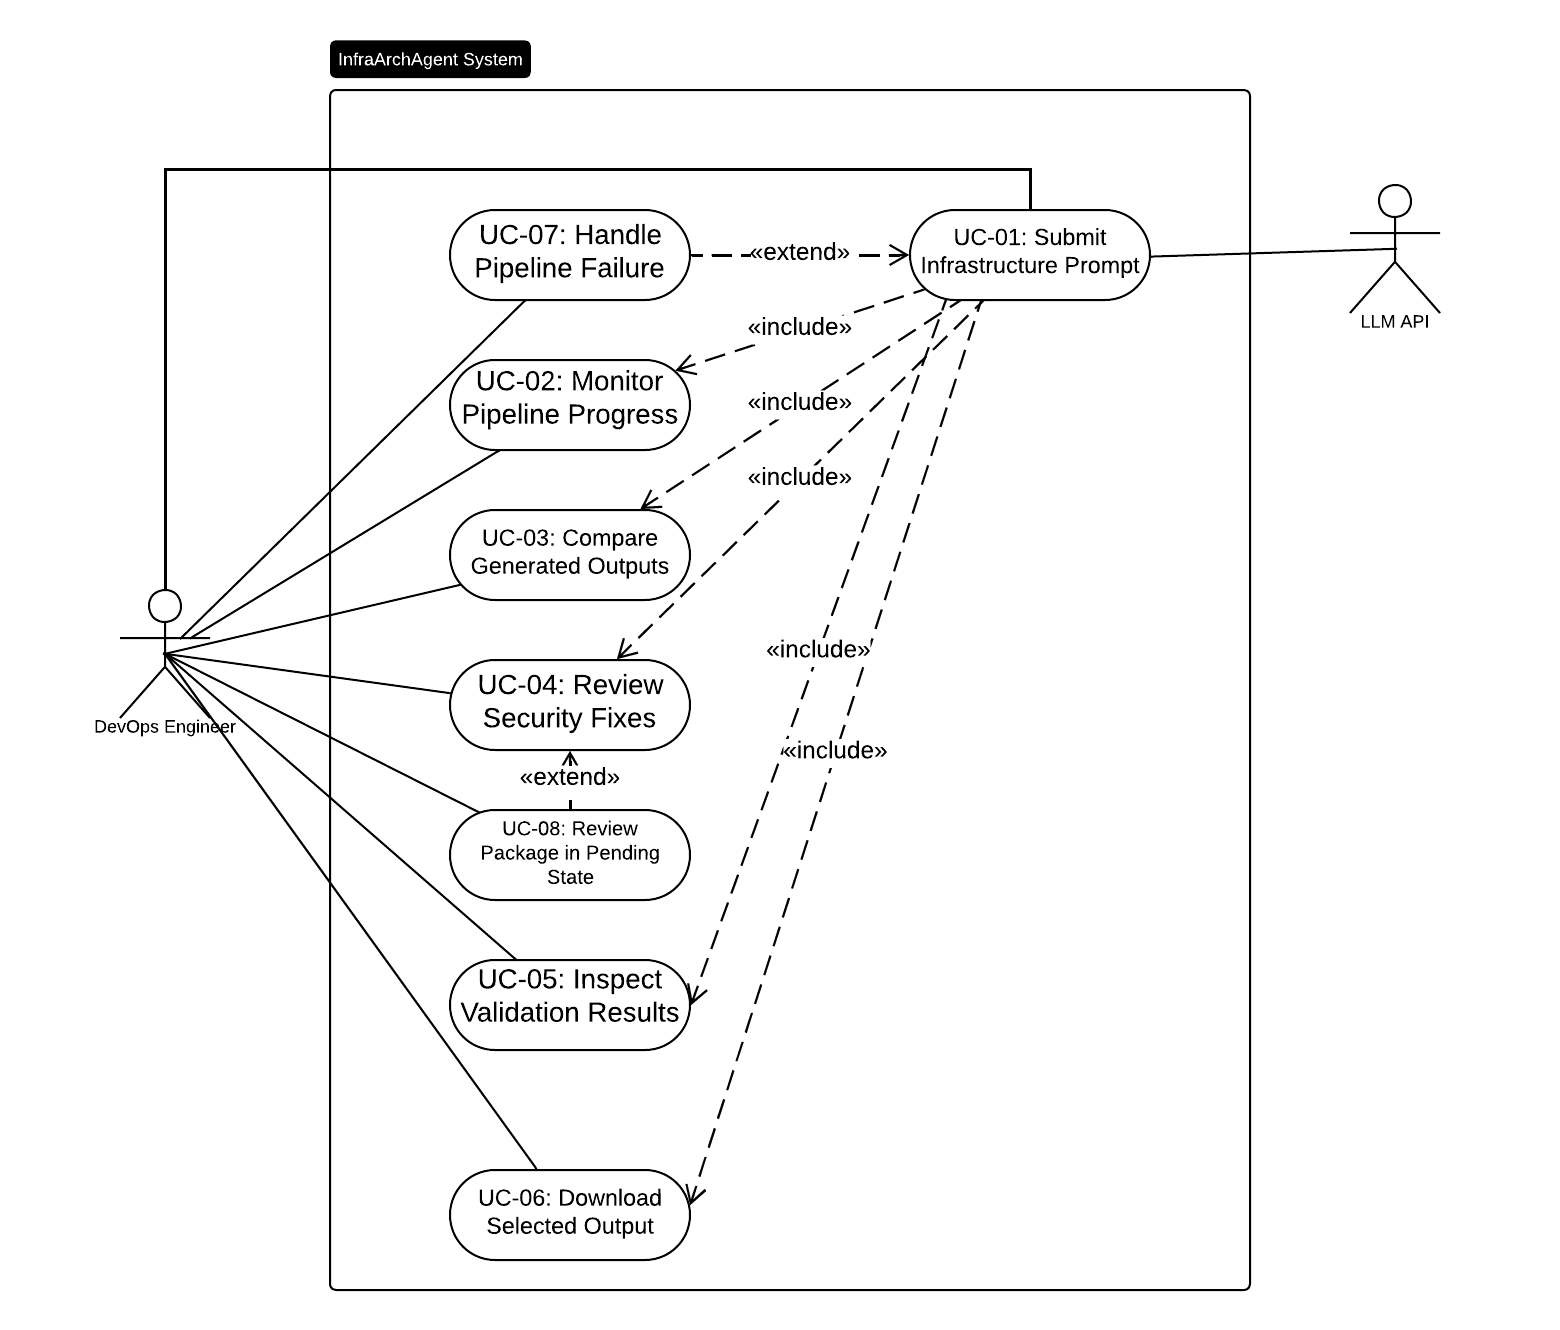
\includegraphics[width=0.85\textwidth]{images/usecase_diagram.png}
  \caption{InfraArchAgent use case diagram.}
  \label{fig:usecase}
\end{figure}

\subsubsection*{UC-01: Submit Infrastructure Prompt}

\begin{description}[leftmargin=3.5cm, style=nextline]
  \item[Actor] DevOps Engineer, LLM API
  \item[Precondition] The system is running and the engineer has a browser
    session open.
  \item[Main Flow] The engineer types a natural-language description and
    submits it. The system validates the input, assigns a run ID, persists
    the request, and hands it to the ArchitectAgent. The LLM API returns
    a structured deployment plan.
  \item[Alternate Flow] If the input contains no infrastructure intent, the
    system rejects it with HTTP 422 and a plain-English explanation before
    invoking any agent.
  \item[Postcondition] A pipeline run is active and the engineer sees the
    progress view update in real time.
\end{description}

\subsubsection*{UC-02: Monitor Pipeline Progress}

\begin{description}[leftmargin=3.5cm, style=nextline]
  \item[Actor] DevOps Engineer
  \item[Precondition] UC-01 completed successfully.
  \item[Main Flow] The engineer watches the real-time progress view as each
    agent transitions through pending, running, and complete states via SSE,
    with every state change appearing within one second.
  \item[Alternate Flow] If an agent fails, its status shows as failed with
    a brief error message; the pipeline continues with remaining agents
    where possible, transitioning to \texttt{partial\_success} if at least
    one generator completed.
  \item[Postcondition] The engineer has a complete picture of which agents
    finished, which failed, and how long each stage took.
\end{description}

\subsubsection*{UC-03: Compare Generated Outputs}

\begin{description}[leftmargin=3.5cm, style=nextline]
  \item[Actor] DevOps Engineer
  \item[Precondition] At least one GeneratorAgent completed and its package
    cleared the SecurityAgent and ValidatorAgent stages.
  \item[Main Flow] The engineer opens the comparison panel showing available
    packages (up to three) side by side, each with a navigable file tree.
  \item[Alternate Flow] If fewer than three generators completed, the panel
    shows only the packages that exist with a note indicating the missing
    variant.
  \item[Postcondition] The engineer has enough information to choose one
    variant for download.
\end{description}

\subsubsection*{UC-04: Review Security Fixes}

\begin{description}[leftmargin=3.5cm, style=nextline]
  \item[Actor] DevOps Engineer
  \item[Precondition] The SecurityAgent completed at least one
    scan-and-remediation pass.
  \item[Main Flow] The engineer opens the diff view for a package and sees
    every line the SecurityAgent changed across all remediation iterations,
    with each change annotated by the Checkov or tfsec rule that triggered
    it.
  \item[Alternate Flow] Unresolved violations appear flagged in a distinct
    colour so the engineer knows they need manual attention before
    deployment.
  \item[Postcondition] The engineer understands what the SecurityAgent
    changed and why, and can decide whether the output is acceptable.
\end{description}

\subsubsection*{UC-05: Inspect Validation Results}

\begin{description}[leftmargin=3.5cm, style=nextline]
  \item[Actor] DevOps Engineer
  \item[Precondition] The ValidatorAgent completed its checks on at least
    one package.
  \item[Main Flow] The engineer reads the validation report alongside the
    diff view; the report lists passed checks, failed checks, and a
    pass/fail summary as separate line items.
  \item[Alternate Flow] Packages that failed validation are not hidden; the
    engineer reviews the report and decides whether to download anyway.
  \item[Postcondition] The engineer knows whether each package is internally
    consistent and what manual corrections may be needed before deployment.
\end{description}

\subsubsection*{UC-06: Download Selected Output}

\begin{description}[leftmargin=3.5cm, style=nextline]
  \item[Actor] DevOps Engineer
  \item[Precondition] The engineer reviewed the comparison panel, diff view,
    and validation report, and chose a variant.
  \item[Main Flow] The engineer clicks the download control; the backend
    returns a ZIP archive of the selected variant's files within two seconds.
  \item[Alternate Flow] If the download fails, the UI surfaces an error and
    lets the engineer retry.
  \item[Postcondition] The engineer has a local ZIP archive of candidate IaC
    files ready for review and deployment at their discretion.
\end{description}

\subsubsection*{UC-07: Handle Pipeline Failure}

\begin{description}[leftmargin=3.5cm, style=nextline]
  \item[Actor] DevOps Engineer
  \item[Precondition] UC-01 was submitted but a non-recoverable error
    occurred: the ArchitectAgent failed after retries, all three generators
    timed out, or the LLM API became unavailable mid-run.
  \item[Main Flow] The system marks the run as \texttt{failed}, persists
    the error details, and surfaces a plain-English failure message
    specifying which agent failed and why. The engineer can correct their
    input or wait for the external dependency to recover and resubmit.
  \item[Alternate Flow] Partial failures where at least one generator
    succeeded transition the run to \texttt{partial\_success} and fall
    under the alternate flows of UC-02 and UC-03 instead.
  \item[Postcondition] The engineer knows precisely what failed, has the
    run ID for debugging, and can decide whether to resubmit.
\end{description}

\subsubsection*{UC-08: Review Package in Pending State}

\begin{description}[leftmargin=3.5cm, style=nextline]
  \item[Actor] DevOps Engineer
  \item[Precondition] A package has entered \texttt{pending\_review}
    (FR-S-07) because it still has unresolved security violations after
    the iteration limit, failed validation (\texttt{invalid}), or has no
    validation report because the ValidatorAgent crashed
    (\texttt{validation\_error}).
  \item[Main Flow] The engineer opens the diff and download view for that
    package, sees why it is under review (outstanding violations, failed
    validation checks, or a missing validation report), and sees the three
    controls described in FR-UI-07. They choose
    one: approve the package as \texttt{production\_ready} despite the
    flagged items, submit optional feedback and request another
    remediation pass, or reject it outright.
  \item[Alternate Flow] If the engineer chooses retry, the package returns
    to the automated remediation loop with a fresh iteration budget and
    may re-enter \texttt{pending\_review} again if it exhausts that budget
    too; there is no limit on how many times this cycle can repeat.
  \item[Postcondition] The package carries a definitive
    \texttt{production\_ready} or \texttt{not\_production\_ready} label
    and is downloadable with that label visible.
\end{description}

% ---------------------------------------------------------------------------
\section{Traceability to the Approved Proposal}
\label{sec:traceability}

\begin{longtable}{@{}p{0.17\textwidth}p{0.13\textwidth}p{0.13\textwidth}p{0.15\textwidth}p{0.17\textwidth}@{}}
\caption{End-to-end traceability matrix.}\label{tab:traceability}\\
\toprule
\textbf{Proposal commitment} & \textbf{Req. IDs} & \textbf{Design evidence} & \textbf{Code evidence} & \textbf{Test evidence} \\
\midrule
\endfirsthead
\toprule
\textbf{Proposal commitment} & \textbf{Req. IDs} & \textbf{Design evidence} & \textbf{Code evidence} & \textbf{Test evidence} \\
\midrule
\endhead

Multi-agent orchestration pipeline &
  FR-A-01--05, FR-G-01--07, FR-P-01--04 &
  Sec.~\ref{sec:sequence-design} &
  Ch.~\ref{ch:implementation} &
  TC-pipeline-01 \\

Security scanning and autonomous remediation &
  FR-S-01--10 &
  Sec.~\ref{sec:sequence-design} &
  Ch.~\ref{ch:implementation} &
  TC-security-01 \\

Interactive UI with real-time visualisation &
  FR-UI-01--07, FR-P-04 &
  Sec.~\ref{sec:ui-design} &
  Ch.~\ref{ch:implementation} &
  TC-ui-01 \\

Competing generator variants &
  FR-G-01, FR-G-03--05 &
  Sec.~\ref{sec:class-design} &
  Ch.~\ref{ch:implementation} &
  TC-generator-01 \\

Pipeline completion within 5 minutes &
  PR-01, PR-05 &
  Sec.~\ref{sec:concurrency-design} &
  Ch.~\ref{ch:implementation} &
  TC-perf-01 \\

Model-agnostic LLM interface &
  FR-I-04, NFR-03 &
  Sec.~\ref{sec:patterns} &
  Ch.~\ref{ch:implementation} &
  TC-adapter-01 \\

Human-in-the-loop production readiness review &
  FR-S-07--10, FR-UI-07 &
  Sec.~\ref{sec:domain} &
  Ch.~\ref{ch:implementation} &
  TC-review-01 \\

\bottomrule
\end{longtable}